% entropy_erasure_notes.tex
\documentclass{article}
\usepackage{amsmath}
\usepackage{graphicx}
\usepackage{caption}

\begin{document}

\section*{Entropy and the Cost of Erasure}

According to Landauer's Principle, the minimum thermodynamic cost of irreversibly erasing one bit of information is:

\begin{equation}
E_{\text{min}} = k T \ln 2
\end{equation}

\noindent where:
\begin{itemize}
  \item $E_{\text{min}}$ is the energy required to erase one bit (in joules),
  \item $k = 1.380649 \times 10^{-23}$ J/K is Boltzmann's constant,
  \item $T$ is the absolute temperature in Kelvin.
\end{itemize}

At room temperature ($T \approx 300$K), the minimum erasure energy is approximately:

\begin{equation}
E_{\text{room}} \approx 2.85 \times 10^{-21} \, \text{Joules}
\end{equation}

\begin{figure}[h!]
  \centering
  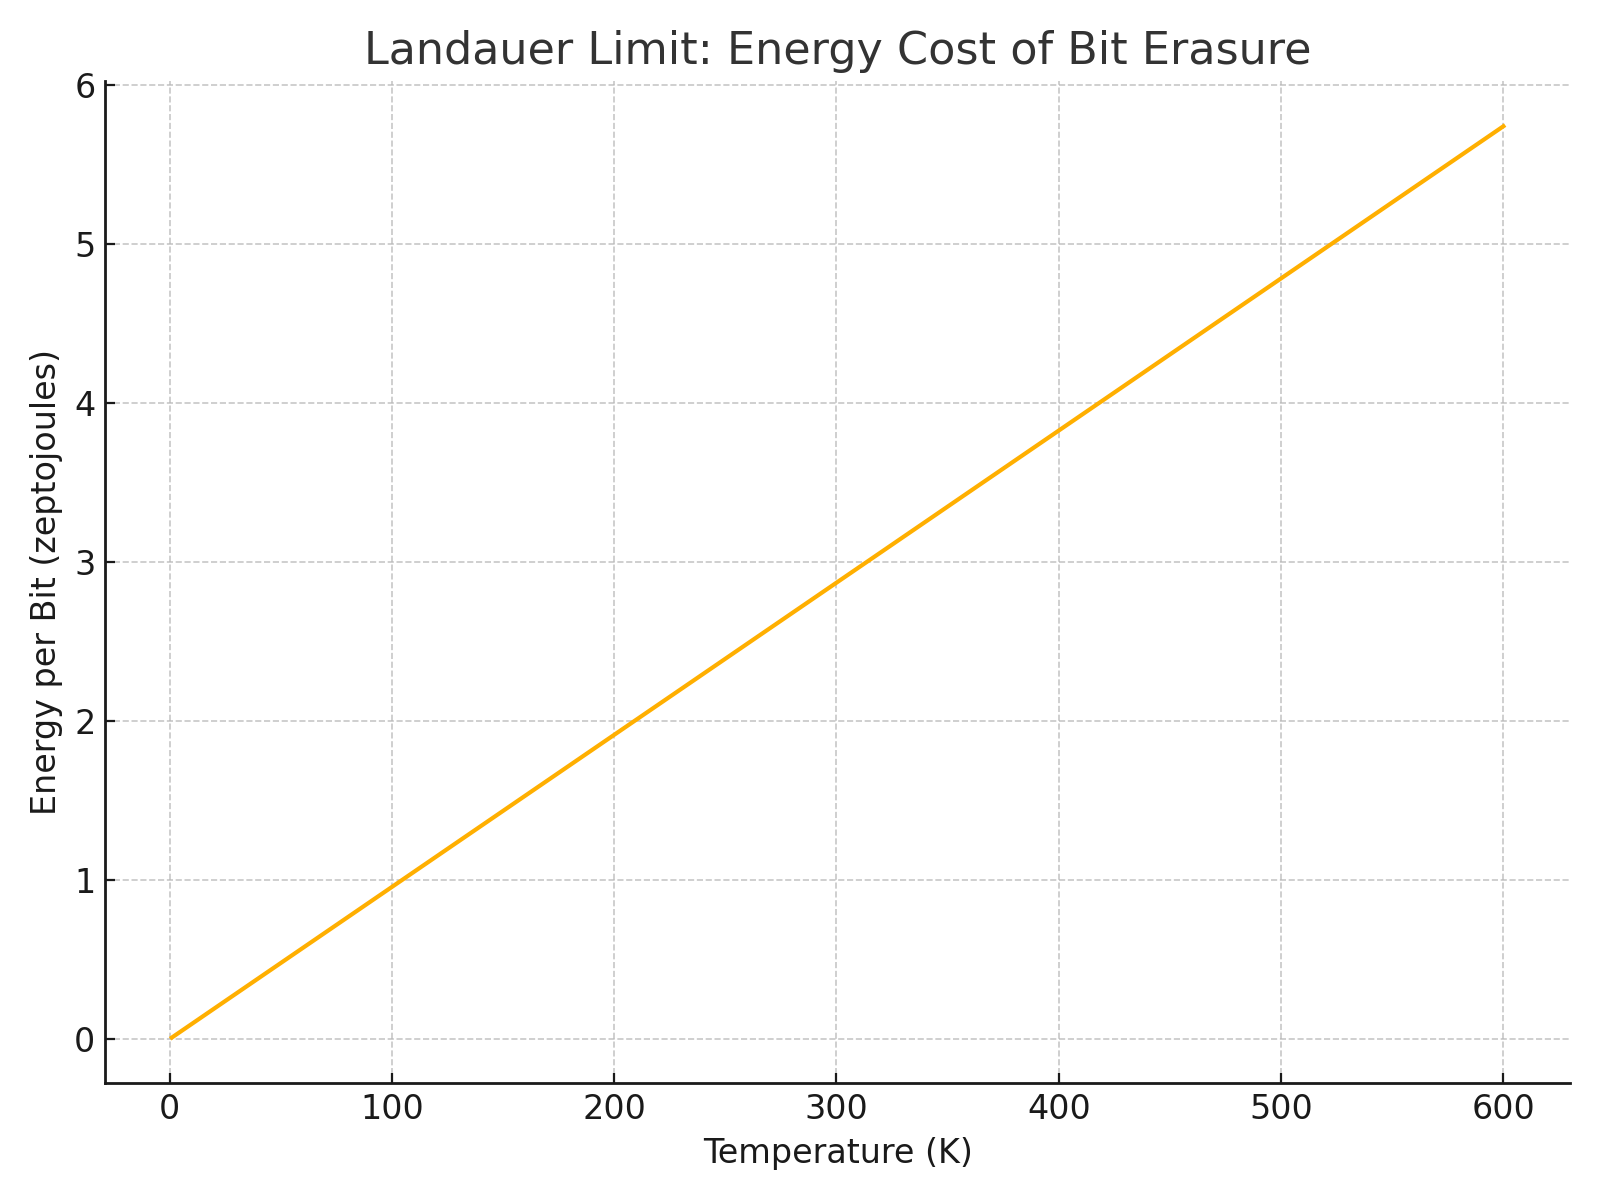
\includegraphics[width=0.75\linewidth]{entropy_erasure_diagram.png}
  \caption{Energy cost of erasure as a function of temperature (Landauer limit).}
\end{figure}

\end{document}

